\documentclass[10pt]{article}
\usepackage{fontspec}
\setmainfont{lmroman10-regular.otf}[BoldFont=lmroman10-bold.otf,ItalicFont=lmroman10-italic.otf,BoldItalicFont=lmroman10-bolditalic.otf]
\setmonofont{lmmono10-regular.otf}
\usepackage[a4paper,margin=16mm,top=14mm,bottom=16mm]{geometry}
\usepackage{multicol,graphicx,xcolor,array,fancyhdr}
\usepackage[hidelinks]{hyperref}
\setlength{\columnsep}{6mm}
\setlength{\parindent}{1em}
\setlength{\parskip}{2pt}
\newcommand{\unk}[1]{\textcolor{red}{\texttt{\scriptsize[U+#1]}}}
\pagestyle{fancy}\fancyhf{}\renewcommand{\headrulewidth}{0.4pt}
\fancyhead[C]{\small }
\begin{document}
% block 0 Picture bbox=[0.0, 0.0, 0.998, 0.9984]
\begin{center}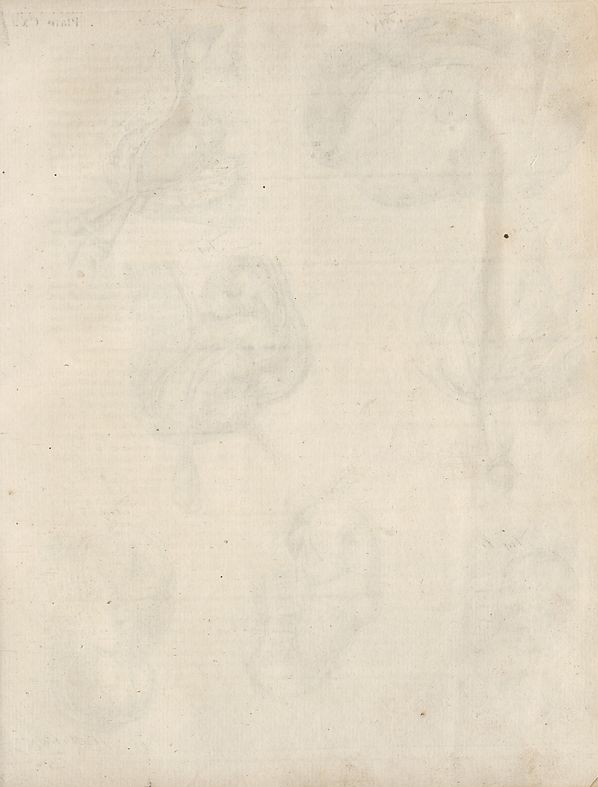
\includegraphics[width=\linewidth,height=0.82\textheight,keepaspectratio]{img/1615-0.jpg}\end{center}
\vfill\par\noindent\rule{\linewidth}{0.4pt}\par
{\scriptsize\color{gray}\noindent Source: Encyclopaedia Britannica scan, text from Parse 3.5 without correction. page\_id: britannica:309f765b1ecc83e0a7f7762e44b4a927a7555443:train:1615 \quad row index: 1615 \quad image sha256: 664ff8d7d9b21a4369b87ea0530c1d02a28e471fbf47881d5d787ac60f0826fd \quad parse model: nvidia/nemotron-3.5-parse \quad parse finish: stop \quad scan: \href{../scans/page-1615-664ff8d7d9b2.jpg}{page-1615-664ff8d7d9b2.jpg}\par}
\end{document}
